\subsection{Elasticsearch Architecture}
To achieve scalability across multiple machines,
the second implementation of query expansion was done using Elasticsearch.
The initial thought was to implement query expansion directly into Elasticsearch's core.
However, during the research phase it was discovered that Elasticsearch has a plugin API.

The query expansion plugin for Elasticsearch is almost identical to the implementation described in subsection \ref{sec:algorithm} and in subsection \ref{sec:lucene}.
Thus, this subsection will only describe the differences.
The differences is mostly how the documents are indexed and how the queries are structured.

\subsubsection{Elasticsearch Plugin API}
Elasticsearch has it's own plugin API\footnote{\url{https://www.elastic.co/guide/en/elasticsearch/plugins/5.2/index.html}}.
This plugin API can be used to extend Elasticsearch's index and query capabilities.
The implementation described in this master thesis creates a plugin which extends the REST API with query expansion.
When a plugin is installed, the installation are done on all the nodes.
The plugin API has two main catogories: core plugins and community contributed plugins.
Core plugins are plugins which are a part of the Elasticsearch project.
These plugins are develop by the Elastic team.
Community contributed plugins, are plugins outside the Elasticsearch project.
These plugins are developed by the community.
When a plugin is installed,
the installation are distributed to all the nodes.
As the installation is distributed,
all the nodes are able to act as a coordination node,
which also makes the plugin API scalable.

Accessing the extended REST API is done sending a POST request to the URL \url{http://localhost:9200/_expansion}.
This URL assumes that the server is running locally and that Elasticsearch's default port 9200 is used.
\texttt{/\_expansion} is the new REST API extension.
To send a query, the POST request need to have a body as shown in listing \ref{lst:rest-api-extension}.
The body consists of a json object with one key value pair.
The key is \texttt{search\_query} and the key is the desired query string.
Query strings with containing multiple terms are divided into separate terms.
The terms are extracted by spliting the query string on the character "space".

\begin{lstlisting}[language=json, caption={The POST request body for the implemented query expansion.}, label={lst:rest-api-extension}]
{
  "search_query": "blue sky"
}
\end{lstlisting}

\subsubsection{Elasticsearch Notes}
- The implementation decribed in this report belongs to the community contributed plugins.

- The implemented plugin extends the current Elasticsearch REST API.

- Architecture with Elasticsearch.

- Elasticsearch plugin to extend the Elasticsearch API.

- Elasticsearch plugin functionality

- Elasticsearch queries in java which are used

\begin{figure}[h!]
\centering 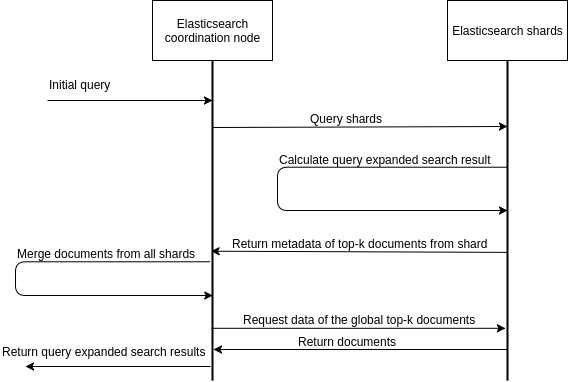
\includegraphics[width=0.9\linewidth]{img/sequence-diagram-elasticsearch.png}
\caption{Sequence diagram for the Elasticsearch implementation.}
\label{fig:sequence-diagram-lucene}
\end{figure}

\subsubsection{Indexing}
Elasticsearch has two different mapping options, dynamic mapping and static mapping.

\subsubsection{Searching}
- Count API
- Maybe faster to use one big request
-
